% SZABLON PRACY MAGISTERSKIEJ - WERSJA 1.0 Z 14 LUTEGO 2010 - MARCIN KULCZYCKI
% Szablon wymaga LaTeXa z zainstalowanymi polskimi stylami
% W skład szablonu wchodzą pliki szablon_mgr.tex i logo_uj.png
% Plik należy kompilować bezpośrednio do formatu .pdf, nie do .dvi (inaczej grafika nie złoży się dobrze)

% Uwaga! Po każdej większej zmianie oraz przed ostatecznym drukiem plik należy przeLaTeXować trzy razy pod
% rząd, aby referencje, cytowania oraz spis treści miały szansę złożyć się we właściwy sposób.

\documentclass[12pt,a4paper]{amsbook}

\usepackage[utf8]{inputenc}
\usepackage{amssymb} % To pakiet z dodatkowymi symbolami matematycznymi
\usepackage{polski} % Te pakiety umożliwiają składanie pracy w języku polskim
\usepackage{graphicx} % Ten pakiet umożliwia umieszczanie obrazków w tekście
\usepackage{indentfirst}	
\usepackage{subfigure}
\usepackage{hyperref}
\usepackage{enumitem}
\usepackage{listings}

%interlinia
	\linespread{1.6}
	
%ustawienia linków (brak obramowania)
	\hypersetup{
	pdfborder={0 0 0 0} 
	}

%brak dzielenia wyrazów
%	\selecthyphenation{nohyphenation}
%	\sloppy

%ustawienia listingów
\lstset{ %
language=XML,                % choose the language of the code
basicstyle=\footnotesize,       % the size of the fonts that are used for the code
numbers=left,                   % where to put the line-numbers
numberstyle=\footnotesize,      % the size of the fonts that are used for the line-numbers
stepnumber=1,                   % the step between two line-numbers. If it's 1 each line will be numbered
numbersep=5pt,                  % how far the line-numbers are from the code
showspaces=false,               % show spaces adding particular underscores
showstringspaces=false,         % underline spaces within strings
showtabs=false,                 % show tabs within strings adding particular underscores
tabsize=2,	                % sets default tabsize to 2 spaces
captionpos=b,                   % sets the caption-position to bottom
breaklines=true,                % sets automatic line breaking
breakatwhitespace=false,        % sets if automatic breaks should only happen at whitespace
title=\lstname,                 % show the filename of files included with \lstinputlisting; also try caption instead of title
escapeinside={\%*}{*)}          % if you want to add a comment within your code
}

\begin{document}

% Strona tytułowa
\begin{center}
\thispagestyle{empty} % Na stronie tytułowej nie chcemy numeru strony

\includegraphics[width=1.5cm, height=1.5cm]{logo_uj.png} % Ta komenda umieszcza na stronie logo UJ

{\large UNIWERSYTET JAGIELLOŃSKI

WYDZIAŁ FIZYKI, ASTRONOMII I INFORMATYKI STOSOWANEJ} \vfill\vfill\vfill\vfill

{\large TOMASZ BOROWSKI \bigskip}

{\Huge SZTUCZNA INTELIGENCJA
W~SYMULATORZE DZIAŁAŃ
ANTYTERRORYSTYCZNYCH}\bigskip\bigskip

{\large PRACA MAGISTERSKA NAPISANA POD KIERUNKIEM

DR HAB. PIOTRA BIAŁASA \vfill\vfill\vfill

KRAKÓW 2012} 
\end{center}


% Streszczenie
\chapter*{Streszczenie}
Niniejsza praca dyplomowa omawia projekt gry symulacyjnej, w~której gracz ma możliwość planowania i przeprowadzania działań antyterrorystycznych. Zastosowane w projekcie algorytmy sztucznej inteligencji, typowe dla gier wideo, zostały uzupełnione algorytmami realizującymi charakterystyczne dla strony konfliktu taktyki. Dokumentacja projektu jest uzupełniona opisem technologi HTML5 Canvas oraz bibliotek JavaScript wykorzystach podczas implementacji.


% Spis treści
\tableofcontents % Spis treści jest generowany automatycznie przez LaTeXa
\let\cleardoublepage\clearpage % To taka mała sztuczka, która nie pozwala LaTeXowi wstawiać pustych stron przed nowymi rozdziałami
\pagestyle{myheadings} \markboth{}{} % Ta komenda pozwala pozbyć się nagłówków stron

% Wstęp 
\chapter*{Wprowadzenie}
Gry wideo, które dotychczas kojarzone były niemal wyłącznie z pojęciem interaktywnej formy dostarczania rozrywki, od wielu lat zdobywają coraz to nowsze pola zastosowań. Przykładem tutaj mogą być gry oparte o zasadę tzw. \emph{edutainment} (w~tłum. \emph{edurozrywka})\footnote{przykładowy serwis z grami edukacyjnymi - http://www.edugames.pl/}. Mają one na celu efektywne przekazywanie wiedzy, dzięki swojemu atrakcyjnemu i rozrywkowemu charakterowi, w takich dyscypliach naukowych jak biologia, fizyka, informatyka lub języki obce. 
Innym polem zastosowań elementów gier jest biznes. Coraz częściej można spotkać się z pojęciem \emph{gamefication} (w tłum. \emph{grywalizacji}) miejsca pracy. Określa ono zestaw technik i narzędzi związanych z grami, które pomagają motywować pracowników do lepszego wykonywania powierzonej im pracy. Dzieje się to poprzez nagradzanie najlepszych pracowników wirtualnymi punktami doświadczenia, osiągnięciami oraz umieszczaniem ich wizerunku na szczytach rankingów\footnote{przykładowa aplikacja bazująca na idei grywalizacji - https://dueprops.com/}.
Wreszcie, możemy mieć również do czynienia z~grami symulacyjnymi. Ich celem jest umożliwienie graczom doznawania wrażeń znanych z~rzeczywistości, a których oni bezpośrednio mogą na codzień nie doświadczać. Wśród takich gier można wyróżnić gry, których celem jest szkolenie użytkowników - np. symulatory lotu - oraz te, których głównym celem jest dostarczenie użytkownikom rozrywki - np. symulator prowadzenia sieci pizzerii.

\begin{figure}
\begin{center}
	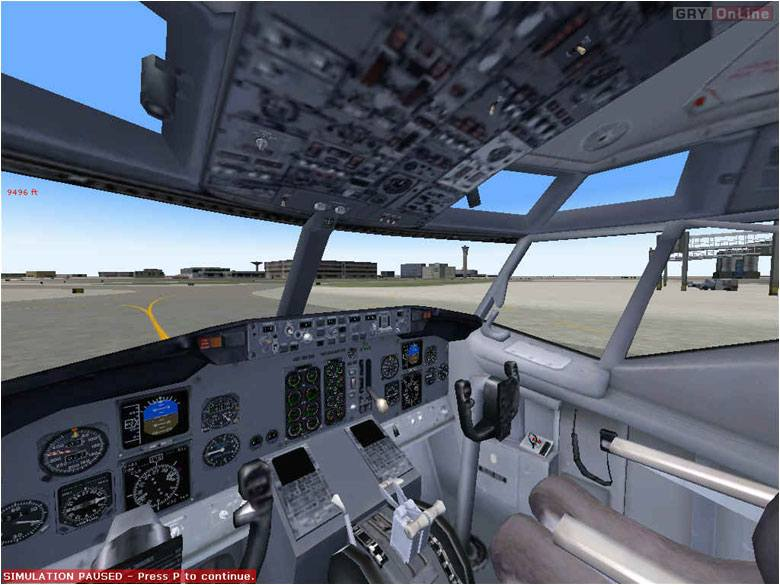
\includegraphics[width=120mm,height=90mm]{images/flightSim}
	\caption{Fligt Simulator 2004 - przykład gry symulacyjnej}
\end{center}
\end{figure}

Niniejsza praca dyplomowa skupia się na projekcie gry symulacyjnej, która odwzorowuje, w dużym uproszczeniu, działania oddziałów antyterrorystyczych podczas szturmu na budynek, zajęty przez wrogie jednostki. Użytkownik grający w tą grę ma możliwość stworzenia schematu budynku, parametryzacji liczby jednostek po obu stronach konfliktu oraz określenia planu działania antyterrorystów. Na podstawie tej konfiguracji gra przeprowadza symulację szturmu na budynek, którą gracz może obserwować.

Realizacja tego projektu obejmuje zaprojektowanie i zaimplementowanie gry oraz omówienie taktyk stosowanych przez strony konfliktu. Zwrócona jest szczególna uwaga na twórcze wykorzystaie algorytmów sztucznej inteligencji, charakterystycznych dla gier wideo. Uzupełnieniem dokumentu jest przedstawienie technologii i bibliotek, które zostały wykorzystane podczas implementacji.




% Literatura:
\bibliographystyle{unsrt}
\nocite{*}
\bibliography{chapters/bibliografia}

% Spisy tabel i rysunków:
\listoftables
\listoffigures

\end{document}
